\chapter{Implementace}
\label{kap_implementace}

Vlastní implementace protokolové brány je v této kapitole vysvětlena v rámci několika částí. Nejprve je popsána
struktura programu, popis tříd, jejich vztah mezi sebou a hlavní funkce, kterou plní. Následuje přehled všech použitých knihoven pro
lepší pochopení dalšího popisu funkce aplikace. Další část tvoří vysvětlení výkonného cyklu programu krok za krokem od spuštění až po
zpracování jednotlivých zpráv. Jsou vysvětleny dosažené výsledky při paměťové optimalizaci a detailně rozebrán systém komunikačních front.
Jako poslední je popsán XML manažer, který byl navržen v předchozí kapitole.

\section{Třídy, vlastnosti a jejich vztahy}
Jak bylo předesláno v předchozí kapitole, při tvorbě byl dáván velký důraz na modularitu jednotlivých součástí programu.
V praxi to znamená, že jednotlivé komunikační jednotky brány nemají tušení, jak ta druhá provádí konkrétní
operace, ale jediným spojením jsou přesně definované struktury obsahující veškeré nutné informace.

Strukturu programu tvoří čtyři třídy:
\begin{itemize}
	\item \textbf{SnmpXmlGate} - hlavní třída, která ovládá běh programu. Při spouštění inicializuje veškeré datové struktury,
	připraví oba komunikační moduly a předá jim řízení.
	\item \textbf{SnmpModule}  - komunikační modul pro zpracování veškerých SNMP požadavků. Plní dvě funkce. První je získávání dat
	z agentů v reakci na dotaz od manažera (resp. XML modulu). Druhou je zpracování asynchronních událostí (Trap, Notification), které
	se na agentech vyskytnou a získané informace zašle definovaným manažerům.
	\item \textbf{Mib2Xsd}	   - transformační třída pro překlad MIB databáze do XML schématu. Netvoří však jenom tento popis, ale zároveň 
	i vytváří finální XML dokument, se kterým pak hlavní program pracuje.
	\item \textbf{XmlModule}   - druhý komunikační modul pro zpracování XML požadavků. Tato třída je vlastní implementací
	navrženého XML protokolu a je pro tuto práci stěžejní.
\end{itemize}

Vzájemné vztahy těchto tříd jsou vyjádřeny na obrázku \ref{obr_impl_vztahy_trid}.

\begin{figure}[htp]
	\begin{center}
		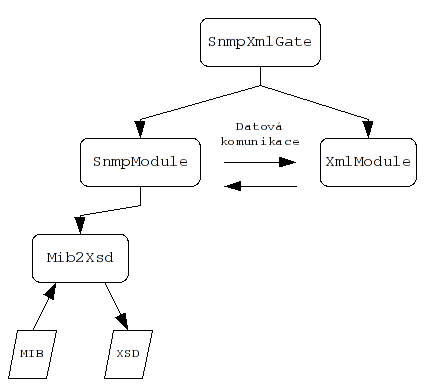
\includegraphics[width=12cm]{obrazky/05_schema_trid.png}
		\caption{Schéma tříd aplikace}
		\label{obr_impl_vztahy_trid}
	\end{center}
\end{figure}


\section{Použité knihovny}
Při tvorbě programu bylo použito několik knihoven, které zajišťují potřebné využívané funkce.

\begin{itemize}
	\item \textbf{ \textit{Xerces-C++ a Xalan-C++} } - knihovny zajišťující manipulace s XML dokumenty, vyhledávání pomocí XPath výrazů (\cite{xerces}, \cite{xalan}).
	\item \textbf{ \textit{Net-SNMP} } - knihovna napsaná v jazyce C, určená pro interpretaci a manipulaci s daty MIB databází, zasílání a 
	přijímání datových SNMP paketů (\cite{net_snmp}).
	\item \textbf{ \textit{libMicroHTTPD} } - volně dostupný HTTP server s podporou použití SSL protokolu při spojení (\cite{libmicrohttpd}).
	\item \textbf{ \textit{libCUrl} } - volně dostupná knihovna určená pro klientskou stranu spojení. Podporuje mimo jiné protokoly HTTP, FTP a
	umožňuje použít i SSL certifikáty pro zabezpečení daného spojení (\cite{libcurl}).
\end{itemize}

Knihovny Xerces, Xalan, libCUrl a libMicroHTTPD využívá XML modul, který má na starosti běh HTTP serveru, operace s XML dokumenty a periodické zasílání
informací.

SNMP modul využívá knihoven Net-SNMP a libCUrl. Druhou jmenovanou využívá vlákno pro zpracování asynchronních událostí (viz dále v této kapitole).


\section{Popis výkonného cyklu}
Detailní popis funkcí jednotlivých tříd je součástí popisu fungování protokolové brány. Jak bylo napsáno v předchozí kapitole,
v rámci běhu programu je několik přesně definovaných fází, ve kterých se systém může nacházet. Tyto jsou vyobrazeny na obrázku \ref{obr_an_beh_programu}.
Některé z těchto fází byly oproti návrhu lehce pozměněny, či rozšířeny, dle potřebného rozsahu splňovaných funkcí.

\subsection{Inicializační fáze}
Je důležité připomenout, že již v návrhu bylo stanoveno jako optimální řešení, že program bude běžet jako démon. Tomu odpovídá
i manipulace s programem. Byl vytvořen spouštěcí skript, který ovládá běh programu - spouští, zastavuje či restartuje (popis instalace,
struktura spouštěcího skriptu a použití je v příloze \ref{kap_uzivatelska_prirucka_brana}).
Jediným vstupním parametrem systému je konfigurační soubor, který je formátován jako dokument XML (přesná struktura souboru se všemi 
povolenými a nutnými elementy je v příloze \ref{kap_struktura_conf_souboru}). Tento obsahuje veškeré nutné informace pro běh systému.

\subsubsection*{Konfigurační soubor}
Informace jsou strukturovány do elementů, kdy každý popisuje jedno spravované zařízení. Každé zařízení je nutné identifikovat
unikátním číslem, které bude použito později při komunikaci s manažery. Dále je nutné specifikovat SNMP přístupové informace
k agentovi:
\begin{itemize}
	\item IP adresu či url
	\item verzi SNMP protokolu
	\item MIB báze, které popisují zařízení
	\item přístupová hesla (community string) pro zápis a čtení
\end{itemize}

Poslední položkou, která je čistě volitelná, je možné definovat manažery, kteří obdrží informace o asynchronních událostech. Každý 
manažer je definován IP adresou či url a portem, na který se budou zasílat jednotlivé zprávy.

Specifickým elementem je definice samotné brány. Tento element obsahuje veškeré informace výše popsány, ale jsou přidány ještě povinné elementy:
\begin{itemize}
	\item \textbf{logFile} - identifikuje soubor, do kterého budou ukládány veškeré textové výstupy
	\item \textbf{snmp}    - obsahuje informace o cestě k souborům definujícím MIB databáze a portu, na kterém budou poslouchány asynchronní události
	\item \textbf{xml}     - definuje xml modul systému. Je zde verze XML protokolu; přístupová práva pro čtení a zápis; cesta k ukládání XSD popisu zařízení;
	porty pro poslouchání požadavků a odesílání odpovědí.
	\item \textbf{security} - obsahuje případné informace o certifikátu a klíči použitém při přístupu přes protokol HTTPS.
\end{itemize}

\subsubsection*{Zpracování a ověření informací}
Poté, co je bezchybně zpracován vstupní soubor, je přistoupeno ke zpracování informací ohledně jednotlivých zařízeních. Tuto fázi má
na starosti třída \textit{SnmpModule}. Nejprve je ověřeno, jestli dané zařízení vůbec funguje a je na něm přítomen SNMP agent. Odešle
se tedy základní požadavek a je očekávána jakákoliv odpověď. Když je agent aktivní, je zařazen do seznamu spravovaných zařízení. Jinak
systém tuto položku vynechá a nebude ji dále brát v úvahu. 

Následuje zpracování seznamu MIB souborů, které popisují nabízené informace. Tyto soubory je nutné vlastnit a přiložit je do dříve specifikovaného
adresáře, odkud si je systém načte a později zpracuje. Jestli všechny soubory existují a jsou načteny, zařízení je finálně "odsouhlaseno" (viz schéma
\ref{obr_impl_inicializacni_faze}).

\begin{figure}[htp]
	\begin{center}
		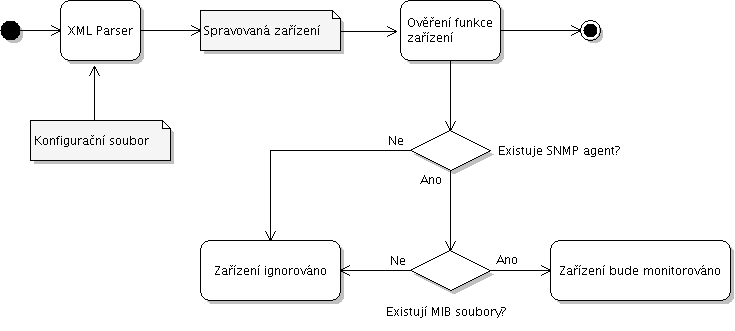
\includegraphics[width=15cm]{obrazky/05_inicializacni_faze.png}
		\caption{Inicializační fáze}
		\label{obr_impl_inicializacni_faze}
	\end{center}
\end{figure}

Po zpracování údajů o všech zařízeních, inicializační fáze končí a systém započne fázi transformační.

\subsection{Transformační fáze}
V této chvíli přebírá úlohu třída \textit{\textbf{Mib2Xsd}}, která se stará o převod MIB popisu databáze do XSD formátu. Pro manipulaci se SNMP je
použita knihovna \textit{\textbf{net-snmp}} (\cite{net_snmp}).

Samotný převod a generování XSD popisu je rekurzivní sestup po jednotlivých uzlech virtuálního stromu MIB databáze.

Pro každé zařízení systém načte všechny specifikované MIB soubory a započne s transformací. Proces se řídí pravidly, které byly definovány v kapitole \ref{kap_xml}.
Jednotlivé uzly jsou popsány svým typem, který obsahuje jejich unikátní identifikační číslo (OID), typ dat a přístupová práva. Samotné uzly jsou pak zařazeny
do stromové hierarchie v rámci dokumentu.

Informace, vztahující se k jednotlivým zařízením, jsou generovány do oddělených souborů. Samostatný soubor
pak obsahuje schéma brány a pouze identifikaci spravovaných zařízení. Tento systém byl vytvořen pro ušetření komunikační zátěže mezi manažerem a bránou.
Bližší popis výhod tohoto přístupu dále v této kapitole.

Oproti navrženému systému mapování MIB do XSD (\cite{macejko_dipl}) byla vynechána nutnost použití prostorů jmen pro jednotlivé MIB databáze. Vzhledem
k tomu, že každý element je popsán unikátním jménem a OID, nedojde při zpracování požadavků ke konfliktu.

Abychom ušetřili procesorový čas, je paralelně s generováním schématu vytvářen i XML dokument, který za běhu slouží k vyhledávání a ostatním potřebným
operacím. Oproti schématu vypadá element specifikující uzel v MIB databázi jako na obrázku \ref{obr_impl_xml_element}.
\begin{figure}[htp]
	\begin{center}
		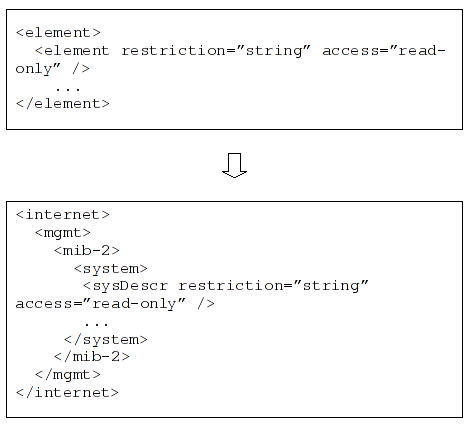
\includegraphics[height=10cm]{obrazky/05_element_xml.png}
		\caption{Příklad struktury hlavního XML dokumentu}
		\label{obr_impl_xml_element}
	\end{center}
\end{figure}

Tento dokument je pak spravován a využíván třídou \textit{\textbf{XmlModule}}.


\subsection{Komunikační moduly}
Po úspěšném zpracování a trasformaci MIB databází je možné přistoupit k inicializaci komunikačních jednotek a otevření síťových spojení k bráně.
V této fázi předává třída \textit{ \textbf{SnmpXmlGate} } řízení třídám \textit{ \textbf{SnmpModule} } a \textit{ \textbf{XmlModule} }. Tyto
moduly pak zajišťují kompletní provoz protokolové brány.

\subsubsection*{XmlModule}
\label{kap_impl_xmlmod}
Dle návrhu programu v kapitole \ref{kap_navrh_systemu} bylo uvedeno, že pro komunikaci mezi bránou a manažery bude použit HTTP server zabudovaný do
aplikace, abychom měli větší kontrolu nad posílanými daty. Proto byl použit nejvhodnější kandidát - microHTTP server (\cite{libmicrohttpd}).
Tento server je napsán v jazyce C. 

Jednotlivá spojení jsou zpracovávána samostatnými vlákny, aby bylo zaručeno co nejrychlejší odbavení požadavků. Funkční cyklus vlánka je znázorněn
na schématu \ref{obr_impl_xmlmod_vlakno}. 
\begin{figure}[htp]
	\begin{center}
		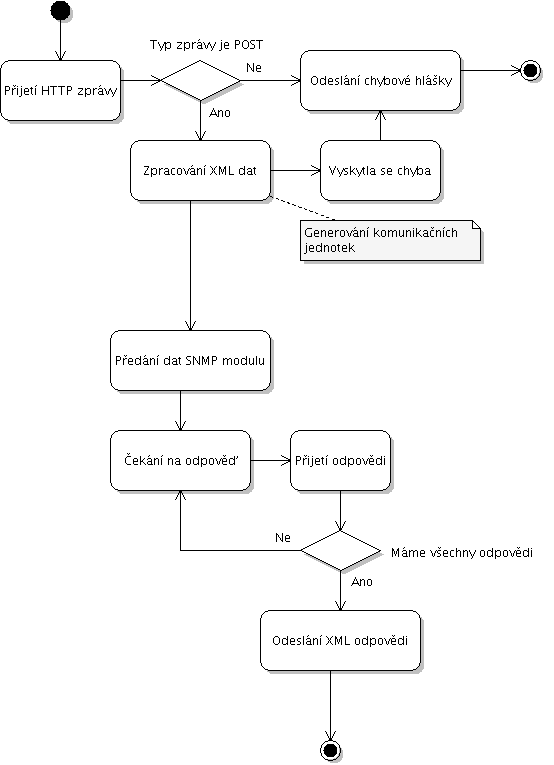
\includegraphics[width=13cm]{obrazky/05_xmlmod_vlakno.png}
		\caption{Zpracování manažerského požadavku}
		\label{obr_impl_xmlmod_vlakno}
	\end{center}
\end{figure}

Nejprve je zpracována HTTP zpráva. Systém operuje pouze s HTTP zprávami typu POST. Jakékoliv GET zprávy jsou zahazovány a zpět klientovi je zasláno
chybové upozornění. Poté je na data použit XML parser, který zpracuje požadavek a ujistí se, že je ve formátu specifikovaném v kapitole \ref{kap_xml}.
Všechny zprávy jsou zpracovávány najednou, aby byla zaručena integrita dat a "atomicita" operací. Více v kapitole \ref{kap_impl_fronta_atomicita}. 
Přesné zpracování jednoho požadavku je popsáno dále v této kapitole.

Pro komunikaci vláken s druhým modulem byly vytvořeny fronty požadavků (pro směr od XML modulu k SNMP modulu)
a jedna odpovědní fronta, ze které se poté vybírají vyřízené požadavky.
Když jsou všechny zprávy v pořádku zpracovány, jsou odeslány do fronty k příslušnému monitorovanému zařízení, nebo jsou rovnou zařazeny
jako odpovědi (obsahují-li chybu, která znemožňuje její další zpracování). Zařazení do fronty k vláknu má na starosti SNMP modul a zároveň
i on probouzí příslušné vlákno ke zpracování požadavků.

Vlákno se následně přesune do čekajícího cyklu, kde kontroluje odpovědní frontu na svoje požadavky do doby, než se dostaví všechny odpovědi. 
Poté vygeneruje odpovědní zprávu a zašle manažerovi. Je na serveru, jak s vlákny poté naloží a jak 
je recykluje. Takzvané zamrznutí a nekonečné čekání vlákna je ošetřeno maximální prodlevou pro jeden požadavek v SNMP modulu. Tím je zaručeno, že
manažer určitě dostane odpověď.

\subsubsection*{Jednotka komunikace}
Než přistoupíme k popisu zpracování jednotlivých XML zpráv, je důležité popsat, jak spolu komunikují oba moduly. Z navrženého protokolu jasně 
vyplývá, že XML manažer komunikuje s bránou tak, jako by to byl samotný XML agent. O protokolu SNMP nesmí vědět. Proto byl již při návrhu
brán zřetel na striktní oddělení těchto dvou protokolů. Pro komunikaci byla navržena struktura, která v sobě obsahuje veškeré informace o
požadavku a odpovědi, ale je protokolově neutrální.

Důležité položky struktury, které oba moduly využívají jsou:
\begin{itemize}
	\item \textbf{typ zprávy} - definuje, jaký požadavek byl vyslán (Get, Set). Dle toho se pak vytvářejí SNMP požadavky na agenta.
	\item \textbf{seznam uzlů} - seznam dvojic (jméno, hodnota), které manažer požaduje.
	\item \textbf{chyba} - identifikace a textová reprezentace chyby, která v celém zpracujícím procestu nastala.
\end{itemize}

Tato struktura pak obsahuje informace o jednom požadavku (Get, Set, Subscribe), který byl v XML zprávě obsažen. 


\subsubsection*{SnmpModule}
Komunikace se SNMP agentama je založen na systému front. Každé monitorované zařízení má na straně protokolové brány k dispozici jedno obslužné vlákno
a frontu zpráv. Schématicky naznačeno na obrázku \ref{obr_impl_snmp_komunikace}. Zpracování a vytváření SNMP zpráv se děje pomocí knihovny \textbf{net-snmp}.
\begin{figure}[htp]
	\begin{center}
		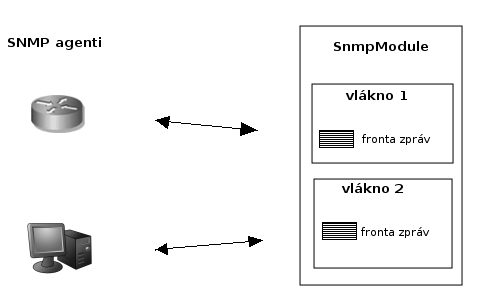
\includegraphics[width=14cm,height=8cm]{obrazky/05_snmp_komunikace.png}
		\caption{Komunikační vlákna brány pro spojení se SNMP agenty}
		\label{obr_impl_snmp_komunikace}
	\end{center}
\end{figure}

Práce komunikačních vláken probíhá v "nekonečném" cyklu. Vstupní informací pro vlákno je identifikační
číslo monitorovaného zařízení, ke kterému patří. S touto informací získá přístup k frontě zpráv a dalším potřebným strukturám, příslušející pouze danému agentovi.
V cyklu se pak opakuje několik dílčích bloků stále dokola.

Vlákno zjistí, jestli v příslušné frontě je přítomen nějaký požadavek na vyřízení. Když není, vlákno se uspí. Jinak vyjme všechny dotazy, tím frontu vyprázdní a
požadavky zpracuje. Tento funkční blok závisí na typu zprávy, která se má vyřídit. 

Zprávy Get a Set, které mají za úkol dostat nebo nastavit hodnotu koncového uzlu stromu, plně korespondují se SNMP. Je vytvořen SNMP packet, do kterého je vloženo
heslo (community string) na základě přístupových práv, které manažer má, je naplněno daty, které se mají nastavit či získat a dotaz je odeslán.

Po přijetí odpovědi jsou data opět z paketu vyjmuta, upravena do požadovaného formátu v rámci komunikační struktury. Pakliže se vyskytla chyba při zpracování, opět
je nastaven chybový příznak ve struktuře, aby manažer dostal informace o problému. Takto vygenerovaná odpověď je poslána do odpovědní fronty a je probuzeno vlákno, které na
data čeká (samotná funkce je ve správě XML modulu).

Složitější je zpracování požadavku na uzel, který není koncový a obsahuje pod sebou celý podstrom dalších uzlů (z hlediska MIB databáze). Poté je nutno opakovat
vytváření paketů a zasílání dotazů ve formě SNMP zprávy GetNextRequest. Až poté, co jsou získána všechna data, je navrácena odpověď klientskému vláknu v XML modulu.


\subsection{Zprávy}
Zpracování jednotlivých druhů zpráv se odvíjí od navrženého modelu. Následuje popis chování systému při přijetí jednotlivých požadavků.

\subsubsection*{Discovery}
Jediným omezením při zpracování požadavku je verze XML protokolu, kterou manažer posílá ve zprávě. Když se rozchází s nastavenou 
verzí v systému, odpovědí je zpráva Publication a chybové hlášení.

Jedním z implementačních požadavků bylo též snížit množství dat mezi manažerem a bránou. Předpokládáme, že brána spravuje
desítky SNMP zařízení. Celý dokument, popisující všechny informace, který je odpovědí na tento požadavek by pak nabyl
obrovských rozměrů. Pro zlepšení protokolu tak systém zašle manažerovi pouze hlavní popis brány s identifikací jednotlivých zařízení, bez ostatních dat.
Manažer si může vybrat, které zařízení chce spravovat a zašle novou zprávu Discovery s volitelným atributem \textbf{objectid}. Po zpracování
mu brána zašle pouze XSD dokument popisující právě to jedno zařízení.

\subsubsection*{Get a Set}
Zpracování těchto požadavků prochází několika fázemi v rámci samotného XML modulu.

Nejprve je nutné zjistit, jestli má manažer právo tyto operace provádět. Heslo, které se zasílá v elementu \textit{message}, určuje, jestli je
povoleno čtení, či zápis. Nastavení hesel probíhá při inicializační fázi, kdy jsou čtena z konfiguračního souboru. Celý přístupový model je
založen na dvou heslech XML protokolu - pro čtení a zápis. Každé SNMP zařízení má pak definována opět dvě hesla, která jsou odlišná od těch prvních jmenovaných.
Systém na základě dodaného XML hesla zjistí, jaké má uživatel práva a použije příslušné SNMP heslo pro požadavek. Může se stát, že mangažer zadal
špatné heslo a systém mu přístup odepře. Pak je odpovědí na tyto požadavky chybová zpráva.

Pokud uživatel má dostatečné oprávnění, je nutné zjistit, zda-li uzly, na které se dotazuje, opravdu existují. Dotazování probíhá pomocí jazyka XPath.
Pokud je dotaz špatně formulován, nebo element neexistuje, systém požadavek zamítne. V druhém případě mohou nastat dvě eventuality.

Element je koncovým uzlem stromu, tj. obsahuje pouze hodnotu danou definovaným typem. Systém takový dotaz interpretuje jako jediný SNMP dotaz GET.
Když se ale jedná o kořenový uzel (obsahuje podstrom uzlů), je nutné tento dotaz interpretovat jako
SNMP zprávu GETNEXT a získat všechny hodnoty daného podstromu (o což se stará SNMP modul).

Jestli bylo požadavkem nastavení určité hodnoty, pak je součástí datové struktury jméno uzlu a příslušná hodnota.

Vygenerovaná komunikační jednotka je vložena do fronty požadavků a pak současně se všemi ostatními odeslána SNMP modulu ke zpracování.

\subsubsection*{Subscribe}
Touto zprávou se manažer upisuje k zasílání pravidelných informací o daném agentovi, nebo tyto údaje mění a maže. Každý takový záznam
se zanese do hlavního XML dokumentu, aby bylo při úpravách a mazání možné vyhledávat pomocí XPath výrazu. Reakce na přidání a úprava
vnitřních struktur je ponechána na speciálním vláknu, které slouží k obsluze daných záznamů. Bližší specifikace dále v této kapitole.

Jediný problém při implementaci nastal v rámci mazání jednotlivých záznamů. Vzhledem k tomu, že v navrženém protokolu je odpovědí
manažerovi zpráva Distribution s daty, která požaduje, nebo chyba, je nutno při smazání záznamu poslat opět zprávu Distribution, ale nyní
prázdnou.

Práva k mazání a úpravám daného záznamu jsou ponechána pouze na znalosti unikátního identifikátoru daného záznamu. 


\subsubsection*{Změny oproti navrženému XML protokolu}
Oproti navrženému XML protokolu bylo nutno udělat několik drobných změn, abychom mohli celý systém implementovat. Jedná se pouze o
minoritní změny - přidání volitelného atributu \textbf{objectid} ke všem typům požadavků, které manažer zasílá. Je to z důvodu
identifiace monitorovaného zařízení, což by bez tohoto zásahu nebylo vůbec možné. Zároveň tento zásah umožňuje ponechat stejnou
strukturu protokolu (co se týče dotazů a odpovědí) pro stroj agenta a brány. 

Abychom nezměnili dosavadní protokol, byl tento atribut zvolen jako volitelný. Jeho nepřítomnost signalizuje, že dotaz je mířen
na samotné zařízení brány, která následně přepošle požadavek na SNMP agenta běžícího na tom samém stroji.


\subsection{Fronty a atomicita požadavků}
\label{kap_impl_fronta_atomicita}
Systém předávání požadavků pomocí front vychází z navrženého protokolu (\cite{macejko_dipl}), ale byl přepracován pro potřeby
této protokolové brány. Navrhovány byly fronty, které by zpracovávaly požadavky dle priority a mamažer by si mohl říci, které
dotazy budou mít jakou prioritu. To bohužel zcela nevyhovuje požadavku zajištění posloupnosti provádění dotazů a tím pádem i 
integritě dat.

Předpokládejme situaci, kdy manažer v jedné XML zprávě zašle dotaz na hodnotu jednoho uzlu s nižší prioritou a zároveň také nastavení
jiné hodnoty s vyšší prioritou (viz obrázek \ref{obr_impl_atom1}). Stalo by se, že při zpracovávání se nastavení provede dříve a manažer by se nikdy nedozvěděl starou hodnotu.
\begin{figure}[htp]
	\begin{center}
		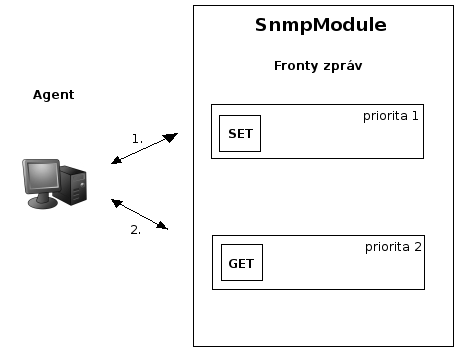
\includegraphics[width=10cm]{obrazky/05_atom1.png}
		\caption{Chyba prioritního zpracování požadavků}
		\label{obr_impl_atom1}
	\end{center}
\end{figure}

Druhým problémem je "atomicita" prováděných operací. Kdyby systém zpracovával jeden požadavek z přijaté zprávy, čekal na odpověď agenta, a pak
přešel na další, mohlo by se stát, že druhý manažer by mohl do tohoto cyklu vstoupit a narušit tak výsledek celé posloupnosti operací.

Proto byl systém přepracován tak, že každé monitorované zařízení má v SNMP modulu jedno obslužné vlákno a frontu požadavků (jak bylo vysvětleno 
dříve v této kapitole). Nyní se v XML modulu zpracují všechny požadavky v rámci jedné zprávy, vygenerují se příslušné komunikační struktury a ty jsou
následně všechny najednou vloženy do příslušné fronty požadavků. Tato funkce je ponechána na SNMP modulu, který zajistí, pomocí systému výlučného přístupu
k dané frontě, aby všechny zprávy tvořily souvislý blok, který bude sekvenčně zpracován.

Je možné, že uživatel v rámci jedné zprávy zašle dotazy na více zařízení. Každé takové zařízení obdrží svůj blok dotazů individuálně.

Předávání odpovědí ze SNMP do XML modulu slouží pouze jediná odpovědní fronta. Do ní se vkládají postupně vyřízené požadavky ze všech zařízení.
Vždy, když je vložena odpověď, jsou probuzena klientská vlákna, zkontrolují frontu a případně si vyberou jim určené odpovědi. Zde by se mohlo zdát,
že bude narušena posloupnost jednotlivých odpovědí v případě, ze komunikujeme s více zařízeními. Tento fakt je ošetřen unikátním identifikátorem každého
požadavku v zasílané zprávě. Odpovědi poté obsahují stejný identifikační řetězec, díky kterému pak manažer pozná, k jaké zprávě se vztahuje obdržená hodnota.

\subsection{Periodické zasílání informací}
Jednotlivými zprávami typu Subscribe se manažer upíše k pravidelnému zasílání informací. Tuto činnost zahrnuje v sobě XML modul, kde na obsluhu těchto
rozesílání je vyhrazeno speciální vlákno. To se stará o veškeré manipulace s jednotlivými záznamy, získávání informací od agentů (pomocí SNMP modulu) a jejich
předávání dále.

Celý systém správy záznamů je založen na hlavním XML dokumentu. Každé spravované zařízení má ve své části element \textit{subscriptions}, kam jsou ukládány
informace o jednotlivých manažerech. Jeden příkladný záznam je schematicky vyjádřen na obrázku \ref{obr_impl_subscript_element}.
\begin{figure}[htp]
	\begin{center}
		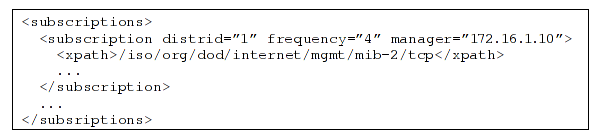
\includegraphics[width=14cm]{obrazky/05_subscr_element.png}
		\caption{Element subscription v rámci hlavního XML dokumentu}
		\label{obr_impl_subscript_element}
	\end{center}
\end{figure}

Každý záznam je identifikován jedinečným číslem a zároveň i zařízením, ve kterém se nachází. Dále element subscription obsahuje informace o frekvenci zasílání, 
url manažera, kam se mají pakety doručovat a v poslední řadě jsou to jednotlivé XPath výrazy pro identifikaci uzlů z databáze dat.
Veškeré úpravy - přidávání, změna a mazání - jsou ponechány ve správě tohoto vlákna.

\subsubsection*{Přidání záznamu}
Když manažer zašle požadavek na zapsání, je obsluhujícím vláknem vytvořen nový element \textit{subscription}, naplněn daty, umístěn do XML dokumentu a 
distribuční vlákno je upozorněno, že nastala změna. Jsou prohlédnuty všechny záznamy a vygenerovány interní datové struktury k správné obsluze.

\subsubsection*{Úprava záznamu}
Vlákno, které zpracovává požadavek klienta, upraví daný záznam v XML dokumentu a oznámí distribučnímu vláknu změnu. To se pak, identicky jako v předchozím případě,
přesvědčí, jaké změny nastaly a upraví interní data.

\subsubsection*{Smazání záznamu}
Záznam, pakliže existuje, je označen jako smazaný, ale vlastní smazání provádí až distribuční vlákno.

\subsubsection*{Zasílání informací}
Vlastní zasílání informací probíhá v jednoduchém cyklu. Jestli není jediný záznam k dispozici, vlákno se uspí a čeká na příchozí zprávy Subscribe. Jsou-li záznamy
k vyřizování, zvolí se nejmenčí časový krok, který je nutný čekat (dle frekvence zasílání jednotlivého záznamu) a vlákno se uspí. Po probuzení je odečten
prospaný čas ode všech záznamů a u těch, které jsou připraveny k vyřízení, předá distribuční vlákno připravené komunikační jednotky SNMP modulu, pro vyřízení
vlastní komunikace. Poté, co dostane odpověď, inicializuje spojení pomocí knihovny \textbf{\textit{libCUrl}} a zprávu Distribution zašle manažerovi na příslušnou
adresu.

Pakliže zpráva nedojde z jakéhokoliv důvodu - manažer je vypnutý, nemůže být zahájeno spojení - je započítán neplatný pokus o odeslání. V momentu, kdy tento počet
překročí stanovenou hranici, je daný záznam smazán a manažer bude muset požádat o nové zapsání zprávou Subscribe. Tento systém je zvolen pro zamezení zahlcení 
distribučního vlákna, které by pak v extrémním případě mohlo spravovat desítky až stovky nefunkčních záznamů, které si nikdo nevyzvedne.


\subsection{Asynchronní události}
Přijímání a zpracování veškerých asynchronních událostí, které agenti posílají na protokolovou bránu, má za úkol speciální vlákno ve správě SNMP modulu.
Funkce tohoto vlákna je přijmout SNMP zprávu (Trap, Notification), zjistit o jaké zařízení se jedná, zvolit všechny manažery, kteří jsou nastaveni pro příjem
XML zprávy Event a zprávu odeslat.

Veškeré nastavení monitorovaných zařízení z hlediska příjemců těchto zpráv je v konfiguračním souboru. Při inicializaci vlákna je zpracován tento seznam pro každé
zařízení.

Vlákno se pak přesune do nekonečného cyklu, kde čeká na definovaném portu na příjem zprávy. Příjem a získání SNMP paketu z příslušného datového spojení je ponecháno
na knihovně \textbf{\textit{net-snmp}}.

Samotné zpracování pak v sobě zahrnuje získání informací o události, inicializaci jednotlivých spojení pomocí knihovny \textbf{\textit{libCUrl}} a zaslání XML zprávy
Event jednotlivým manažerům. Z navrženého protokolu vyplývá povinnost získat potvrzení o doručení paketu. To za nás vykoná transportní protokol TCP, který je knihovnou libCUrl
použit. Není-li možné paket doručit - manažer neexistuje či je vypnutý - pak je informace zahozena a brána se již o tento fakt nezajímá.


\section{Paměťové optimalizace}
Hlavním bodem zadání této práce není jenom implementace protokolové brány, ale i optimalizace využití operační paměti. Při vývoji se objevily dva body, kdy bylo nutno 
vymyslet optimalizaci systému. Oba dva body se opírají o manipulaci a uložení XML dokumentů, které v paměti zabírají velký prostor.

Prvním je správa XSD schémat, která popisují jednotlivá monitorovaná zařízení. Každou příchozí zprávou Discovery se manažer dotazuje na tato popisná schémata. Bylo by, pro 
rychlejší odbavení požadavku, snadnější uchovávat celá schémata v paměti. Za předpokladu, že jedno schéma zabírá minimálně několik stovek kB (při použití pouze standardní
sady MIB databáze) paměti a že bychom spravovali několik desítek zařízení, mohla by se nutná paměť rozrůst do desítek MB. Proto se každé takovéto schéma ukládá do
souboru na pevném disku a v případě potřeby je soubor načten a zaslán manažerovi. Časový rozdíl je relativně malý v porovnání s množstvím paměti, která se ušetří.

Druhým bodem je minimalizace velikosti hlavního XML dokumentu, který je udržován po celou dobu chodu protokolové brány v paměti. Není dost dobře možné, bez zásadních změn
navrženého protokolu, sdílet části virtuálního stromu dat. Proto vycházejme z předpokladu, že na spravované síti reálně existují identická zařízení, která používají
stejnou sadu MIB databází. Zároveň je tu druhý předpoklad, že v rámci běžné sítě se nepoužívá mnoho jednotlivých zařízení, která by v rámci SNMP protokolu nabízela ke správě odlišná data.
Kdybychom měli u každého takového zařízení spravovat v hlavním XML dokumentu celý datový strom, nebylo by možné udržet tento v paměti a zároveň na něm provádět
efektivně vyhledávání a jiné operace.

Proto byl stanoven takzvaný sdílený systém, který se dotýká i prvního bodu. Zařízení, která mají v konfiguračním souboru nastavenu stejnou sadu MIB databází, jsou prohlášena za shodná, co se týče
dat, a je vytvořeno pouze jedno popisné XSD schéma a do hlavního dokumentu je uložen pouze jeden takovýto strom. Ostatní zařízení mají nastaveno identifikační číslo shodného agenta.
Při jakémkoliv požadavku na vyhledání elementů ve stromu či popisné schéma, je vyhledáváno právě v tom jediném sdíleném stromu, nebo navráceno jediné sdílené schéma.

Tímto nejenom, že v rámci předpokladů ušetříme aktuální operační pamět, ale zároveň i místo na pevném disku, kde jsou popisná schémata ukládána. Z hlediska splnění zadání bylo tedy
dosaženo optimálního řešení.


\section{XML Manažer}
Nedílnou součástí implementační části je vytvoření XML manažera, který by dovolil otestovat protokolovou bránu v praxi. Vzhledem k tomu, že není náplní práce vytvořit plnohodnotného
klienta, který by postkytoval veškeré uživatelské pohodlí grafické aplikace a jiných možných aspektů, byl vývoj omezen na tvorbu aplikace ovládané pomocí příkazového řádku.

K tvorbě manažerské aplikace byly použity knihovny:
\begin{itemize}
	\item \textbf{ \textit{libCUrl} } - zajištující klientské spojení s HTTP serverem na bráně (\cite{libcurl})
	\item \textbf{ \textit{libMicroHTTPD} } - HTTP server použitý pro příjem asynchronních událostí a periodické distribuce dat (\cite{libmicrohttpd})
	\item \textbf{ \textit{libargtable2} } - knihovna zajišťující pohodlné zpracování vstupních parametrů programu (\cite{argtable})
\end{itemize}

Aplikace funguje ve dvou možných formách - aktivní nebo pasivní (kompletní instalační a uživatelská příručka je v příloze \ref{kap_uzivatelska_prirucka_manazer}).

\subsubsection*{Aktivní mód}
V tomto módu je součástí vstupních parametrů URL protokolové brány, XML heslo a soubor, který obsahuje jednotlivé požadavky, které chce
uživatel provést. Systém načte vstupní soubor a pakliže je vše bez chyby zpracováno, vygeneruje XML zprávu dle navrženého protokolu. 

Tuto zprávu pak odešle a čeká na odpověď. V případě, že byla odeslána zpráva Subscribe a jsou tedy očekávány periodické dodání informací,
je spuštěn HTTP server a jako v předchozím případě, aplikace čeká na odpovědi.

Při ukončení tohoto čekání zašle aplikace XML zprávu, kterou zruší veškeré Subscribe záznamy, které předtím odeslala.

\subsubsection*{Pasivní mód}
Tento mód slouží jako takzvaný "poslouchací". Při něm se pouze aktivuje webový server a očekávají se příchozí zprávy ohledně asynchronních událostí.
V tomto módu nelze odesílat žádné požadavky.
